\section{Multi-unit PRA}
\label{sec:multiUnitPRA}

Given the model described in Sections ~\ref{sec:RISMC_MU_modeling} and~\ref{sec:plantRomModeling} 
along with the set of stochastic parameters Section~\ref{sec:plantStochasticModeling} we have 
simulated $10^6$ accident scenarios using RAVEN Monte-Carlo sampling
capabilities. For each simulation, we have collected the binary output (OK or CD) from 
each model/ROM (i.e., all PWRs and SFPs).

The use of ROMs instead of the actual codes allowed us to generate this very large 
database of data which helped us to visualize and understand timing and sequencing of events at 
the unit level.

Figures~\ref{fig:histFlex1}, ~\ref{fig:histFlex2} and ~\ref{fig:histFlex3} give an example of pdf
of the actual EPE actuation time for Unit 1, Unit 2 and Unit 3 respectively. 
The presence of three distinct site recovery strategies and the possibility to involuntary align
EDGS from Unit 2 to Unit 1 strongly affect the time convolution of such timing of events. 

\begin{figure}
    \centering
    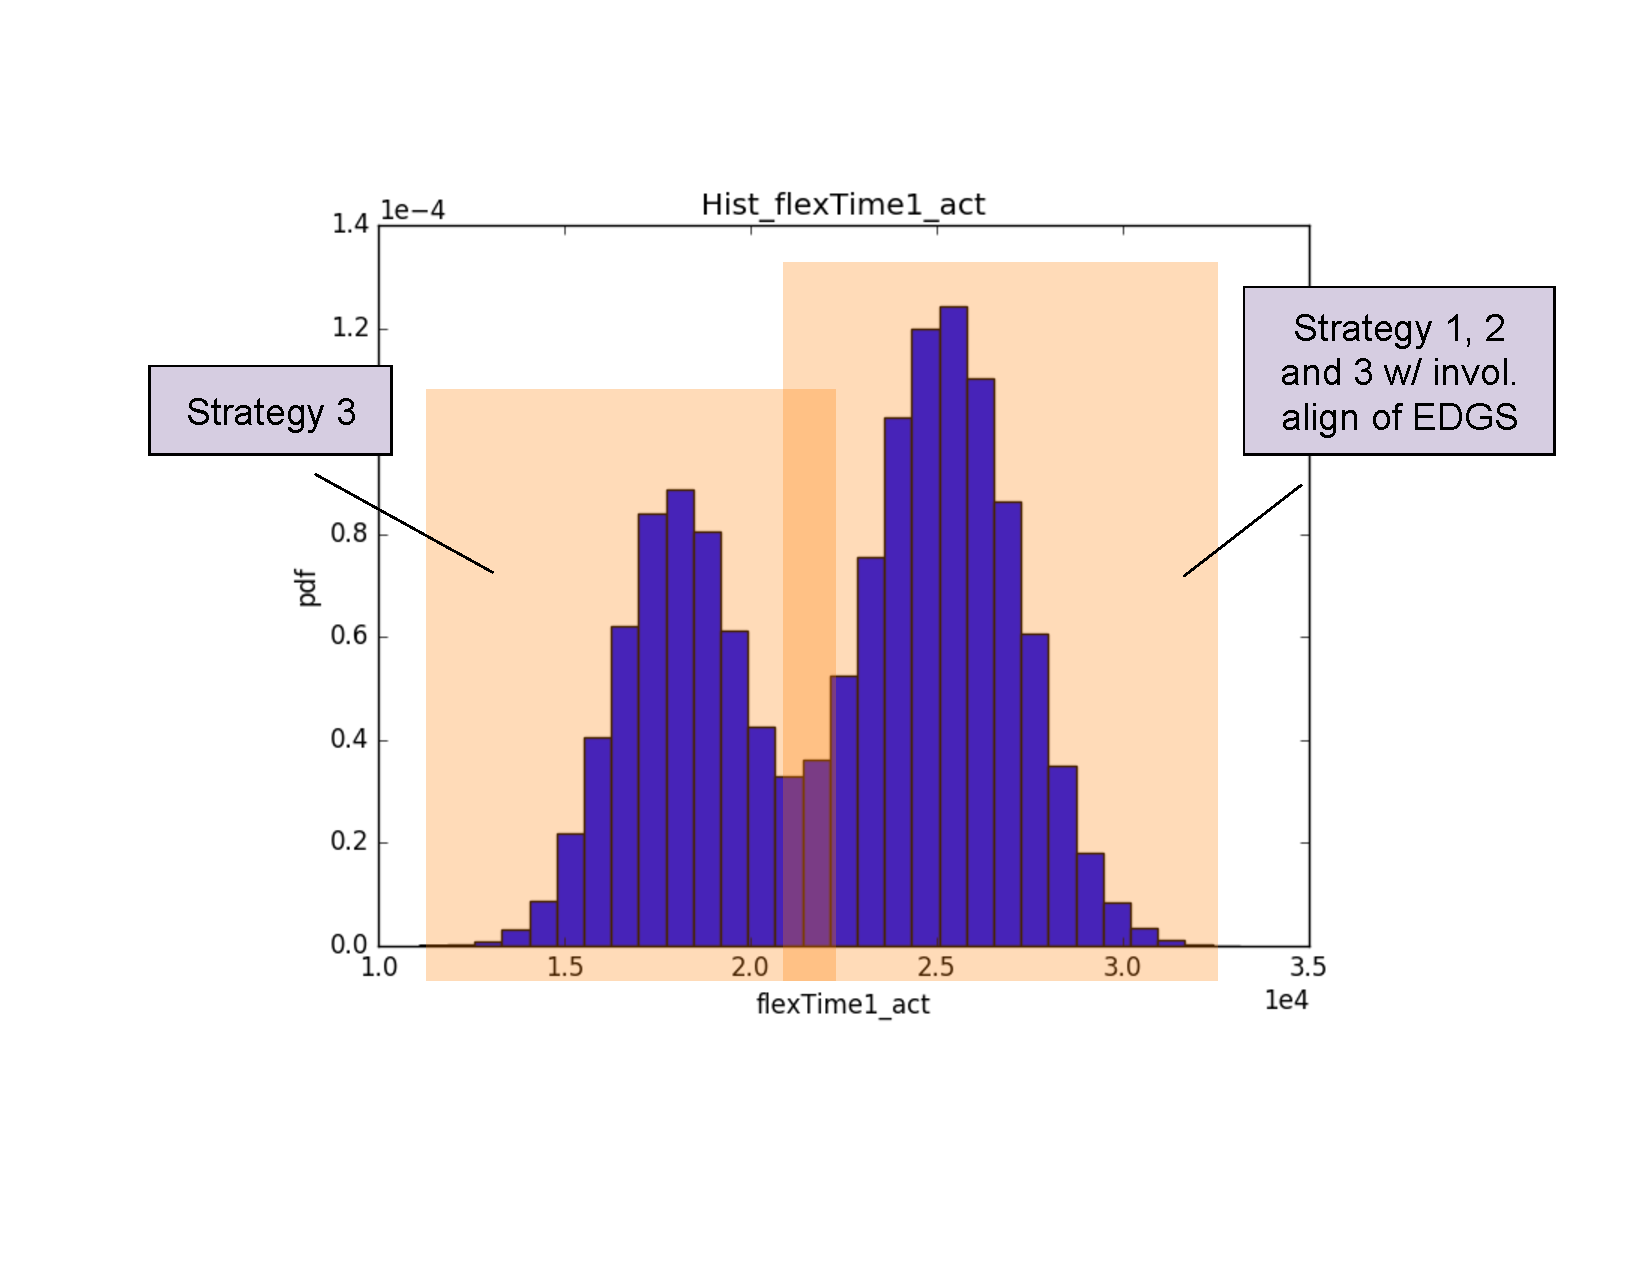
\includegraphics[scale=0.5]{histFlex1.pdf}
    \caption{Histogram of EPE actuation time for Unit 1}
    \label{fig:histFlex1}
\end{figure}

\begin{figure}
    \centering
    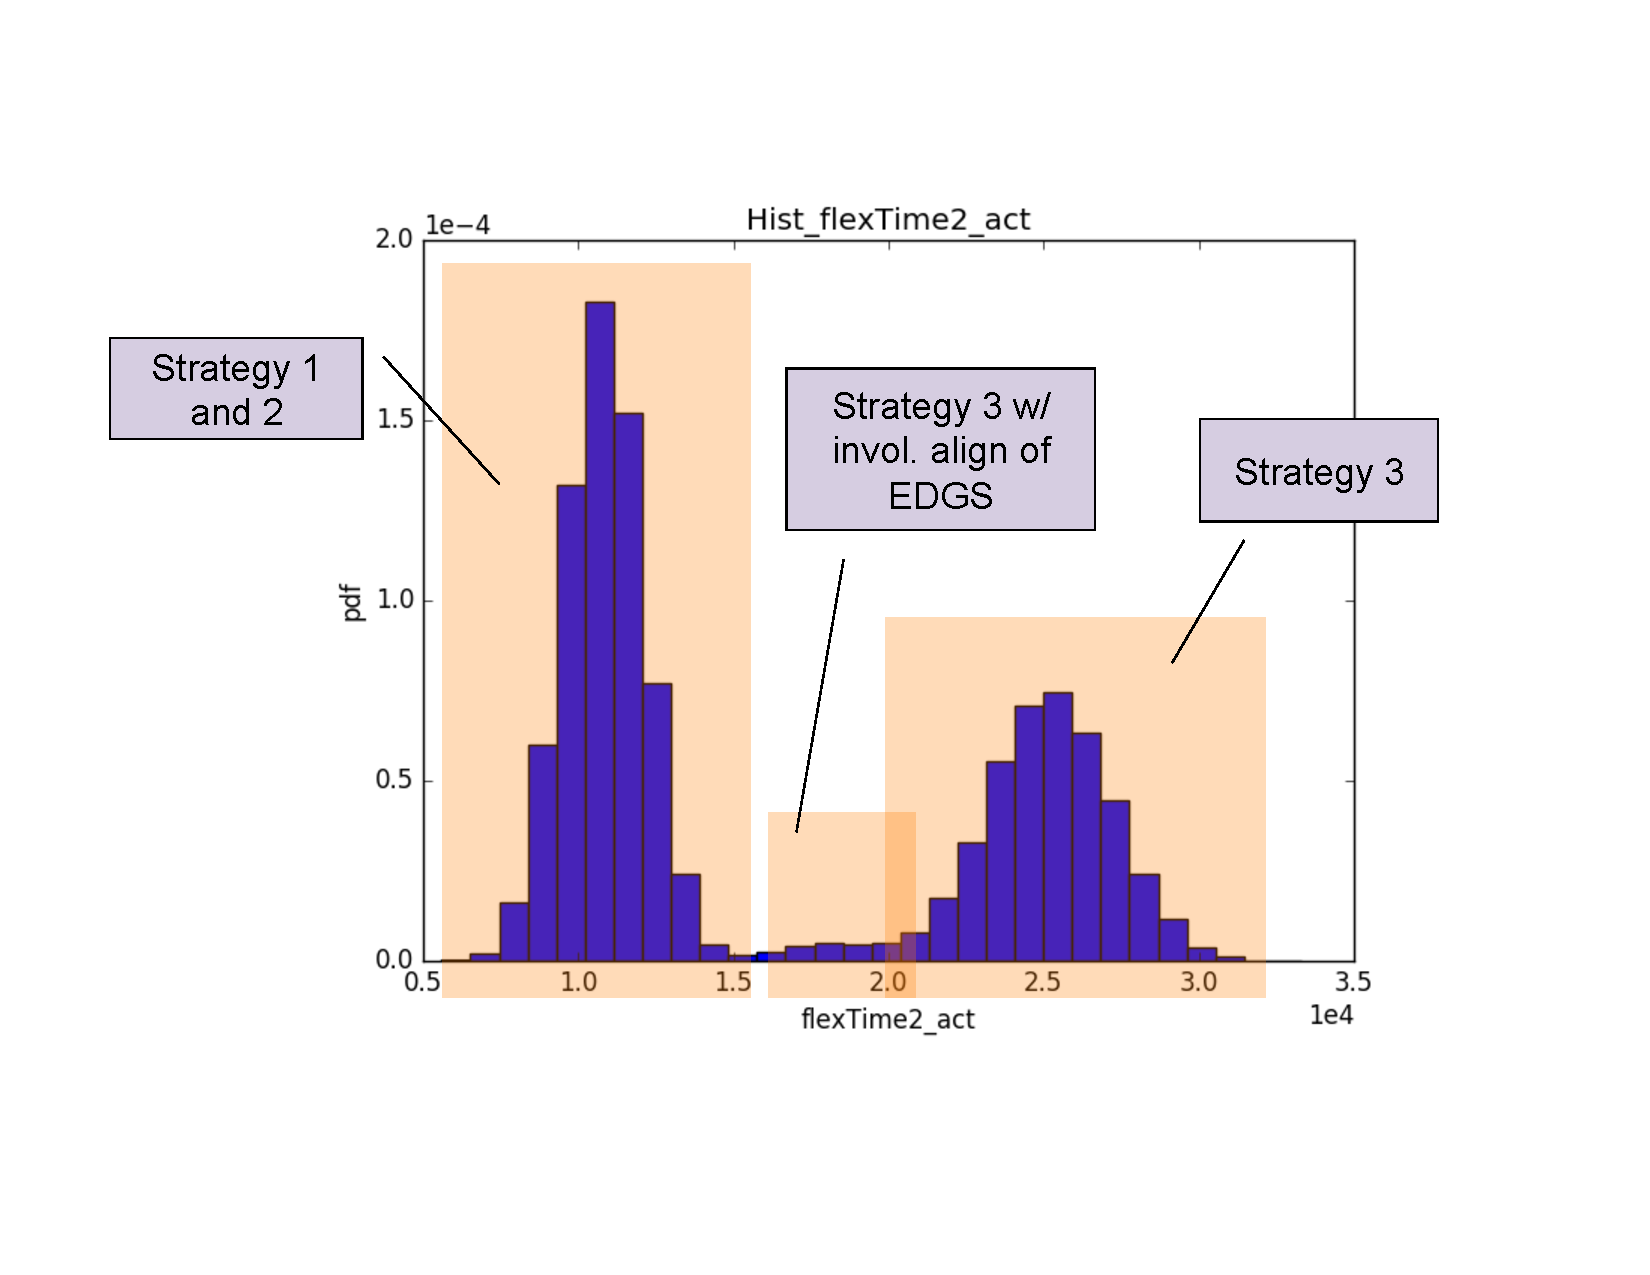
\includegraphics[scale=0.5]{histFlex2.pdf}
    \caption{Histogram of EPE actuation time for Unit 2}
    \label{fig:histFlex2}
\end{figure}

\begin{figure}
    \centering
    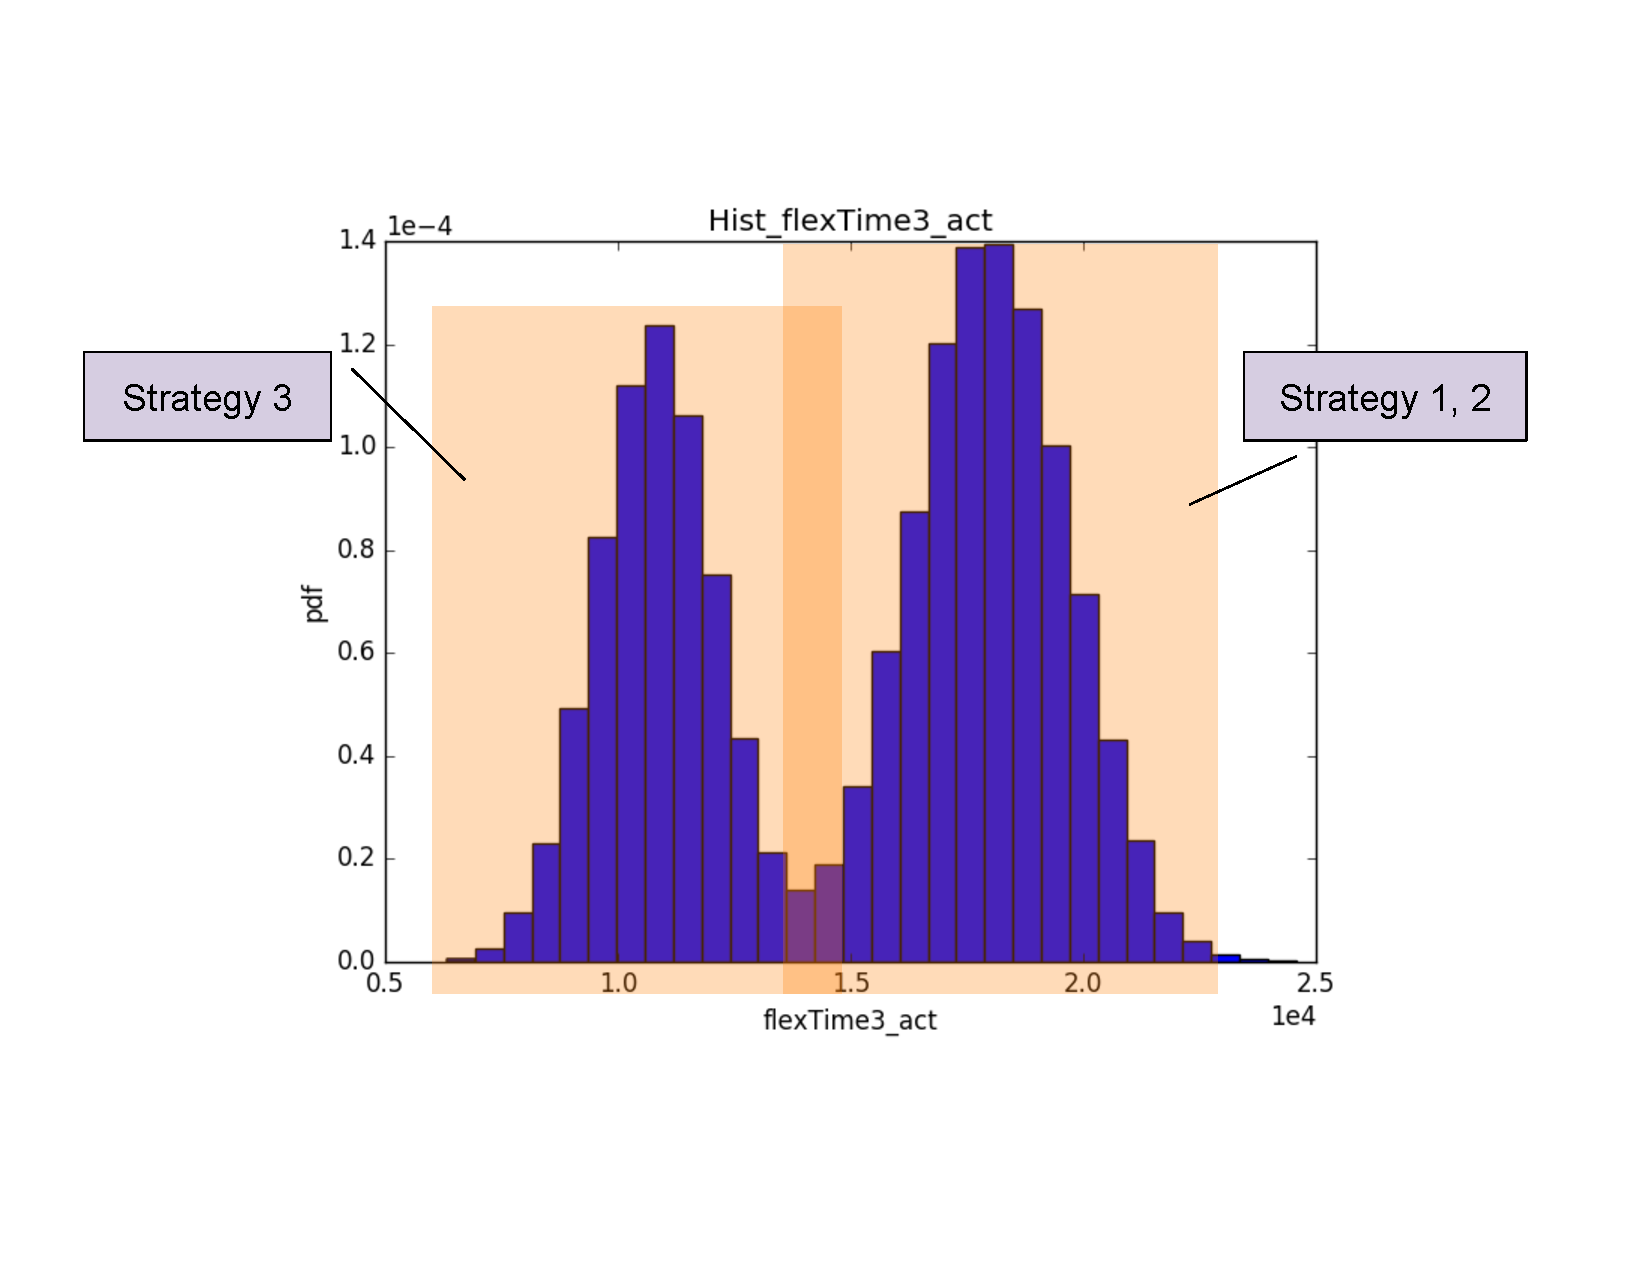
\includegraphics[scale=0.5]{histFlex3.pdf}
    \caption{Histogram of EPE actuation time for Unit 3}
    \label{fig:histFlex3}
\end{figure}

\begin{figure}
    \centering
    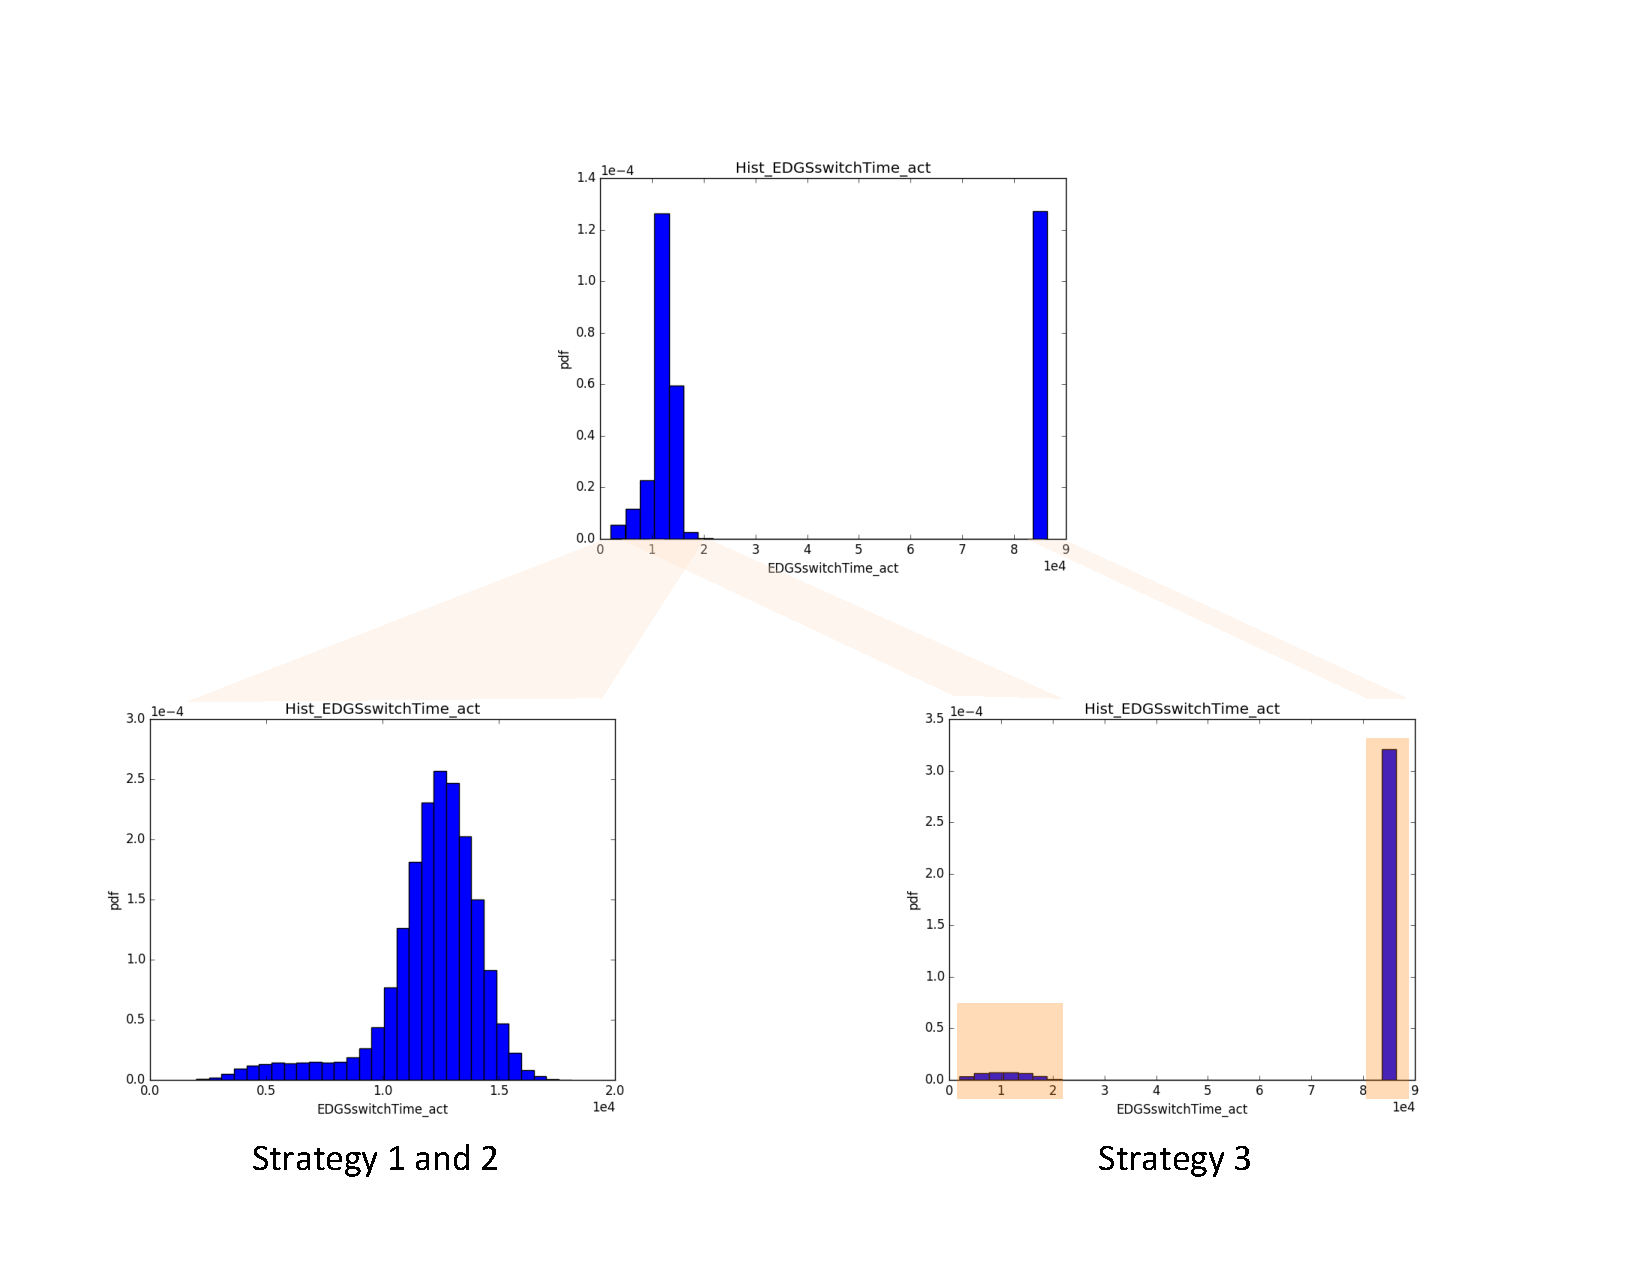
\includegraphics[scale=0.5]{EDGSswitch.pdf}
    \caption{Histogram of EDGS switch time}
    \label{fig:EDGSswitch}
\end{figure}